\section{Time Delay Measurement Between H1 and L1 Detectors} \label{sec:4} 
\subsection{Method: Cross-Correlation}

A genuine astrophysical gravitational-wave signal must appear in both detectors with a time delay consistent with the light travel time between Hanford and Livingston (approximately $\pm 10$ ms). To measure this delay, the whitened and bandpass-filtered strain data from H1 and L1 were cross-correlated.

Given two discrete time series $h_H(t)$ and $h_L(t)$, the cross-correlation is defined as

\[
C(\tau) = \sum_{t} h_H(t) \, h_L(t+\tau),
\]

where $\tau$ is the time lag. The lag that maximizes $C(\tau)$ provides an estimate of the relative arrival time between the two detectors.

Prior to correlation, the Livingston data were multiplied by $-1$ to account for the relative detector orientation, which can invert the signal phase for certain sky locations.

The analysis was performed on a $\pm 1$ ms window around the merger time.


\begin{figure}[h]
	\centering
	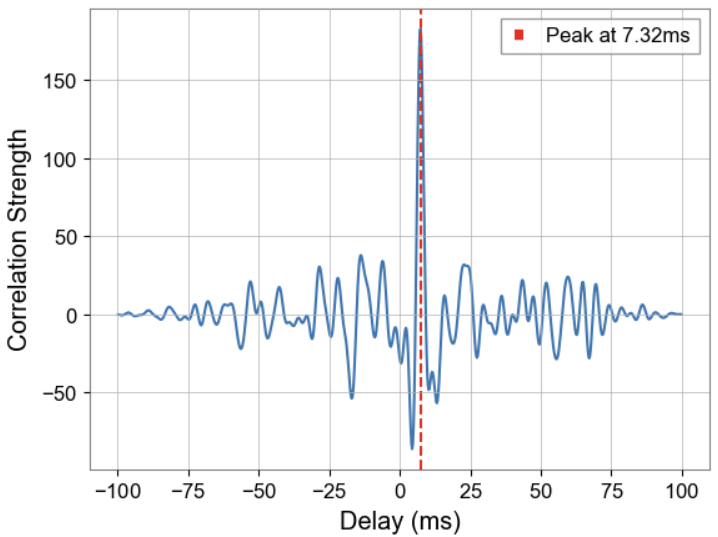
\includegraphics[width=0.6\textwidth]{figure/cross_correlation_peak}
	\caption{Cross-correlation between H1 and L1 showing a clear peak at the measured time delay.}
	\label{cross correlation}
\end{figure}

The cross-correlation exhibits a clear and statistically significant peak corresponding to a relative delay of

\[
\Delta t \approx \textbf{7} \ \text{ms}.
\]

This delay is well within the physically allowed range set by the 3000 km separation of the detectors. The sign of the delay indicates the direction of propagation across the detector network.

The presence of a sharp correlation peak strongly supports the interpretation of a coherent astrophysical signal observed by both interferometers.


\subsection{Off-Source Validation}

To assess the significance of the measured delay, the same procedure was applied to an off-source segment located 200 seconds away from the merger time. In this case, no dominant correlation peak was observed, and the inferred delay was consistent with random noise fluctuations.

\begin{figure}[h]
	\centering
	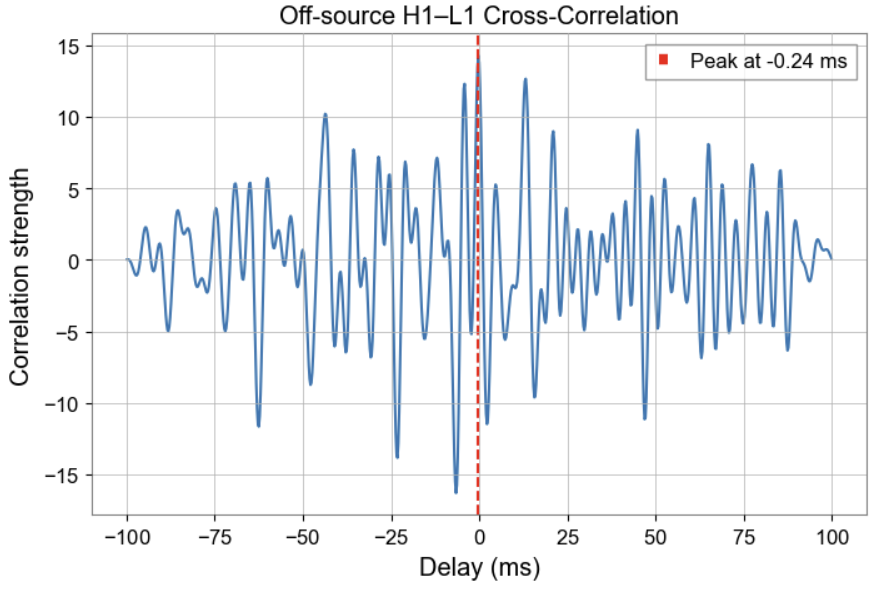
\includegraphics[width=0.6\textwidth]{figure/offsource_correlation}
	\caption{Cross-correlation in an off-source window showing no significant peak.}
	\label{off sourc cross correlation}
\end{figure}

The contrast between the on-source figure \ref{cross correlation} and off-source \ref{off sourc cross correlation} results demonstrates that the measured inter-detector delay at the merger time is not a generic feature of the noise but is associated with a transient coherent signal.

\subsection{Key Result}

The coincident detection of a transient signal in both detectors with a physically consistent time delay constitutes the first independent confirmation, within this analysis, that GW150914 is not a local instrumental artifact but a genuine gravitational-wave event.
